\documentclass[12pt, letterpaper]{article}
\usepackage[utf8]{inputenc}
\usepackage[margin=0.75in]{geometry}
\usepackage{amsmath, amssymb}
\usepackage{titlesec, enumitem}
\usepackage{graphicx}
\usepackage{caption}
\usepackage{float}
\setlength\parindent{0pt}
\title{Minimax Quiz Solutions}
\author{Team Chairun}
\date{November 29, 2020}

\begin{document}

\maketitle

1. Suppose we have the following payoff matrix for $A$ in a zero-sum game where $A$ moves first: \\
\begin{table}[H]
\centering
\begin{tabular}{|c|c|c|}
    \hline
    & $B$ Cooperates & $B$ Defects \\
    \hline
    $A$ Cooperates & -1 & 4 \\
    \hline
    $A$ Defects & 2 & 2 \\
    \hline
\end{tabular} \\
\end{table}
Assuming both players play optimally, what is $A$'s optimal strategy and payoff? \\
1A. If $A$ chooses to cooperate, they receive a payoff of $\min(-1, 4) = -1$. If they defect, they receive a payoff of $\min(2, 2) = 2$. Then $A$ should defect and get the payoff of $2$. \\\\
2. What is the purpose of using a heuristic in minimax? \\
2A. A heuristic allows us to cut off the search at a given depth and still evaluate the game state to a number. Without it, we would have to search until the end of the game for every single search we do. \\

3. Suppose a game where each player takes 2 turns in a row. How would the minimax algorithm change? \\
3A. Normally, in the maximizing function we call the minimizing function and vise versa. However in this game, we would instead call the maximizing function twice each time, then call the minimizing function twice. Alternatively, we could search two moves deep in every maximizing/minimizing call. \\

4. In the Tactics Solver assignment, there are some situations where the engine is unable to find the solution without a very high depth, regardless of the depth of quiescence search. What kind of situations might cause this? \\
4A. Since quiescence search only looks at checks and captures, moves which don't fall under these categories are overlooked. For instance, pawn pushing and promoting (which sometimes cannot be stopped) is neither of these so the Tactics Solver will be unable to find the solution without a depth high enough to see the actual promotion occurring. \\

5. Why would iterative deepening be used instead of breadth-first search in minimax? \\
5A. While both solutions have the same asymptotic runtime, breadth-first search uses too much memory to be realistically implemented for higher depths. \\

6. Why can't we just search at a fixed depth until our alotted time runs out instead of using iterative deepening? \\
6A. Any minimax search done at a certain depth is not effective unless we finish the entire search at that depth. This is because the next move we decide to look at could be the best one, so if we stop before completing the search then we could miss a better move that would appear later on. \\
\newpage
7. Fill in the node values calculated by minimax in the tree below and cross out branches pruned by alpha-beta pruning. $\Delta$ are maximizing and $\nabla$ are minimizing.
\begin{figure}[H]
    \centering
    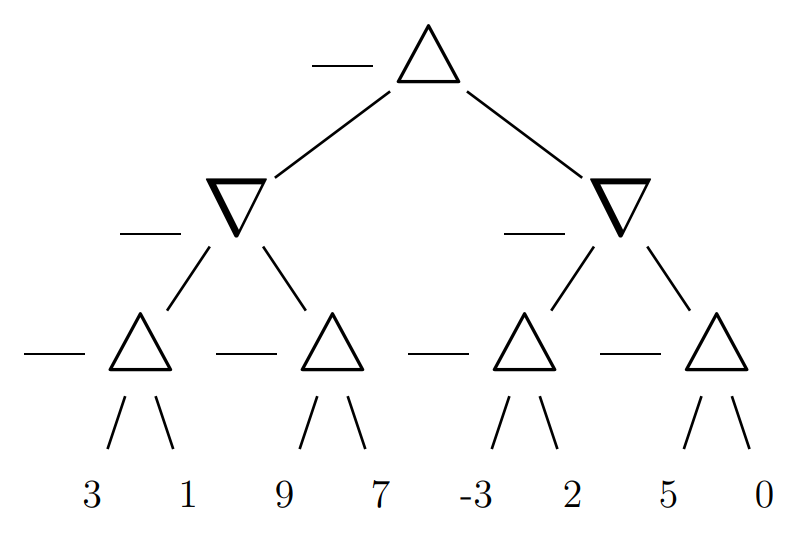
\includegraphics[scale=0.3]{minimax-prob.png}
    \caption*{From CS 61B Fall 2016 Midterm 2}
\end{figure}
7A.
\begin{figure}[H]
    \centering
    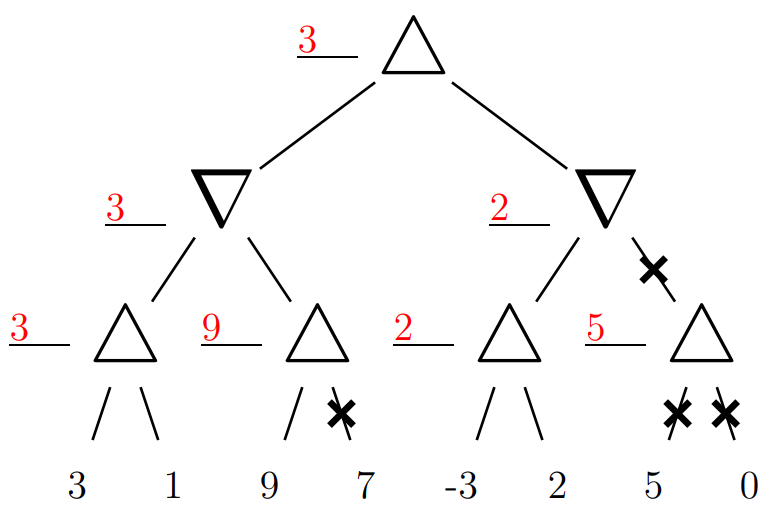
\includegraphics[scale=0.3]{minimax-sol.png}
    \caption*{From CS 61B Fall 2016 Midterm 2}
\end{figure}
8. Fill in values for $a$ and $b$ so that the crossed out branches shown below would be pruned by alpha-beta pruning.
\begin{figure}[H]
    \centering
    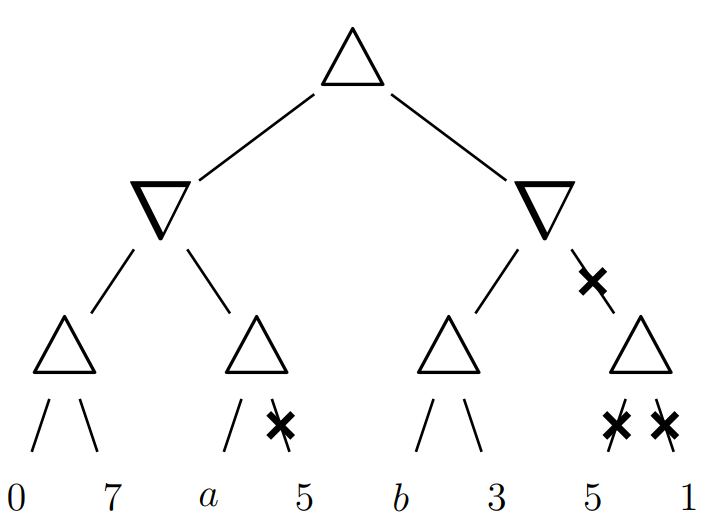
\includegraphics[scale=0.3]{alpha-beta-prob.png}
    \caption*{From CS 61B Fall 2016 Midterm 2}
\end{figure}
8A. $a > 7$ so that its subtree is pruned. $b < 7$ so that the subtree next to it is pruned since we have guaranteed a value of $7$ in the left subtree. \\ 


9. Suppose you have the functions findMax and findMin as written in the slides. You wish to find the best move for a game, but for some reason the heuristic you have gives payoffs which are flipped. How do you find the best move for the player which normally would be maximizing? \\
9A. Instead of findMax call findMin with the same inputs. \\

10. In chess, there are positions which are referred to as "sharp," where the position is volatile and the evaluation can change very drastically depending on the moves played. Would alpha-beta pruning run more quickly in a "sharp" position or a non-"sharp" position relative to conventional minimax with no pruning? \\
10A. Alpha-beta pruning would most likely run more quickly in the sharp position, since the drastic evaluation changes would result in some moves being far superior to others, meaning we could likely prune with a much higher frequency. \\

11. Suppose a game with a branching factor of 7. How many states do we search if we begin a minimax search with no pruning of depth 3? \\
11A. $7^3 = 343$ states. \\

12. Explain possible drawbacks to the following heuristic for Connect-4, where the goal is to get $4$ pieces in a row: $(\text{Reds in a row}) - (\text{Blacks in a row})$. \\
12A: The heuristic does not recognize that having a blocked line of pieces is useless.
\end{document}